\chapter{Designing and modeling the system}\label{ch:designing_and_modeling}
This chapter includes the UPPAAL models in conjunction with corresponding UML
diagrams describing the implementation done in Ada. The UPPAAL models are used
for the validation and verification of the system that it meets the real-time
requirements set on the system. The connection from the UPPAAL models to the
UML diagrams presented here are to show that the implementation corresponds as
close as possible to the models verified.

For presentation purposes only the messages concerning basic functionality
during component and service discovery is presented in this chapter. After the
initial discovery and configuration process have been done the system continue
in normal operation mode with an extra set of SPA message types. Detailed
sequence diagrams over the component and service discovery process is shown in
section \ref{sec:discovery_process}.

\section{First iteration}
The first UPPAAL models were created after designing the basic structure of the
system. Each application will do the same thing which is receive, handle
and send messages. The difference between the applications is which
messages each application understands and which messages the application will
ignore. A processing node will at most have one CAS, one SM-L and one LS
but can have any number of applications running next to them. This inspired the
first iteration of UPPAAL models that the application automaton should be
possible to instantiate multiple times in UPPAAL but the other more specific
models can be used only ones. The basic component overview is shown in figure
\ref{fig:processing_node_overview} which is what the UPPAAL model is to
resemble as close as possible.

\begin{figure}[h]
    \centering
    
\includegraphics[width=\textwidth]{figures/processing_node_overview}
    \caption{A Processing Node overview with core SPA parts.}
    \label{fig:processing_node_overview}
\end{figure}

\subsubsection{A basic application}
The basic functionality of an application is that it should be able to identify
itself on the network, share its capabilities and request information from
other applications. An application is only connected to one subnet at a time.
The limitied functionality of an application makes for a basic two-layered
design where the upper-layer alter its behaviour depending on incoming
message types and the lower layer is only responsible for sending and receiving
messages on its subnet. The application sends out Local\_Hello message during
boot-up and receives a Local\_Ack response, all messages are modeled as
transition between different states. It then receives a logical address with
the Assign\_Address message. As final step it receives a Probe\_Request from
the Lookup Service to share its capabilities. Figure
\ref{fig:iteration1_application} shows the UPPAAL model.

\begin{figure}[h]
    \centering
    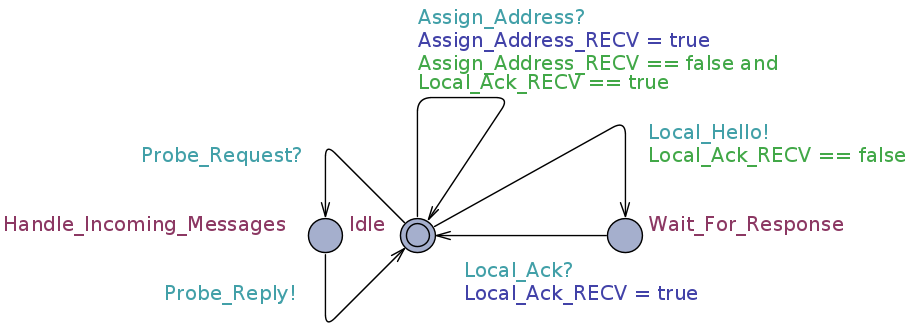
\includegraphics[width=\textwidth]{figures/iteration1_application}
    \caption{UPPAAL model of a first iteration application.}
    \label{fig:iteration1_application}
\end{figure}

\subsubsection{Central Addressing Service (CAS)}
Specifics for the CAS is that it assigns an address to itself so no need for
processing of Assign\_Address messages. As addition to basic application
functionality the CAS sends out address block to the requesting subnet
managers. Figure \ref{fig:iteration1_cas} shows the UPPAAL model.

\begin{figure}[h]
    \centering
    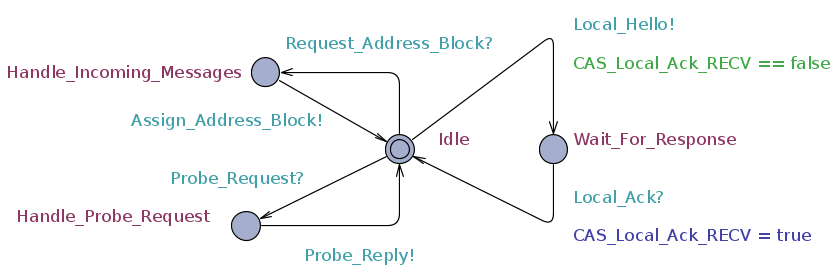
\includegraphics[width=\textwidth]{figures/iteration1_cas}
    \caption{UPPAAL model of a first iteration CAS.}
    \label{fig:iteration1_cas}
\end{figure}

\subsubsection{Lookup Service (LS)}
The additions the LS brings in is the processing of Request\_LS\_Probe,
Probe\_Reply and Probe\_Request messages, for service discovery purposes.
Figure \ref{fig:iteration1_ls} shows the UPPAAL model.

\begin{figure}[h]
    \centering
    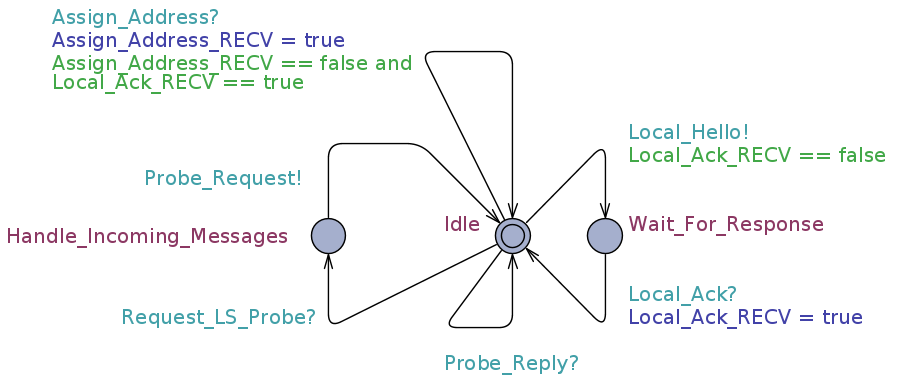
\includegraphics[width=\textwidth]{figures/iteration1_ls}
    \caption{UPPAAL model of a first iteration LS.}
    \label{fig:iteration1_ls}
\end{figure}

\subsubsection{Local Subnet Manager (SM-L)}
In contrast to the other components the Subnet Manager manages most of the
interaction done in the subnet. It's responsible for answering all Local\_Hello
messages during component discovery and replying with an acknowledgement as
well as with an logical address assignment. As a last step it tells the LS to
send out Probe\_Requests to all active components on the subnet.Figure
\ref{fig:iteration1_sm_l} shows the UPPAAL model.

\begin{figure}[h]
    \centering
    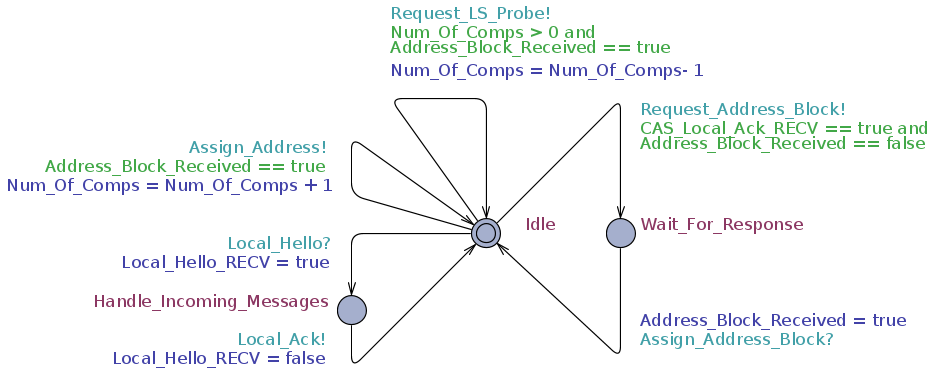
\includegraphics[width=\textwidth]{figures/iteration1_sm_l}
    \caption{UPPAAL model of a first iteration SM-L.}
    \label{fig:iteration1_sm_l}
\end{figure}


\subsubsection{First iteration conclusions}
The CAS, LS and SM-L have specific functionality so they can only be used ones
when setting up a complete network of automata. The application model can be
instantiated multiple times as was the goal. At this level of abstraction
everything looks fine though the main goal with the UPPAAL model is to be able
to verify that the system behaves as aspected and can't reach unknown states or
deadlock. As the first iteration of models only shows the boot-up process it
will eventually reach deadlock when everything is set up. This is a drawback
as it doesn't relate very well with the actual design of the system, that can
have different applications come online and go offline at any time, not just
during initial boot-up. This calls for another iteration and improvement of the
different UPPAAL automata.

Before heading to the second iteration it's time to take a closer look at the
UPPAAL automata and see what other parts need improvements, as it should
resemble the actual system as much as possible.

First of is the current automata use transitions to model sent and
received messages. When a transition is taken to send a message the different
automata takes the transition to responed immediatly afterwards. This is more
or less an event-based system which is not how the system should behave.
Instead the second iteration of UPPAAL models should be modeled as a
time-triggered system so responses can be sent later on.

The models only works with a set of eight different message types and in the
current design of the UPPAAL models it's hard to add another type of message.
If possible the second iteration should make it possible to add and remove
specific message types with ease.

As a third improvement time invariants should be added to the different
automata so verification of real-time requirements can be done.

\section{Second iteration}
To improve the UPPAAL models a more detailed design is required of the system.
From the first iteration it's clear that the basic application can be designed
in a generic fashion. The CAS and LS is more specific instantiations of the
basic application and the SM-L has substantial differences. For easier
maintanence of the models during the second iteration it would be valuable if
the UPPAAL models could created in a modular way. Two main models would be the
"basic application" and the "SM-L".

Figure \ref{fig:iteration2_uml_component_overview} shows the component overview
after the second iteration. The design of the interfaces between the components
makes it easy to interchange which message types each "running task"
(application) can handle and how it communicates. A simple application that is
only connected to one subnet does not need the Routing component. The Routing
component is specifically created for the SM-L to be able to route traffic
within its own subnet and to other subnet managers over other types of subnets.

\begin{figure}[h]
    \centering
    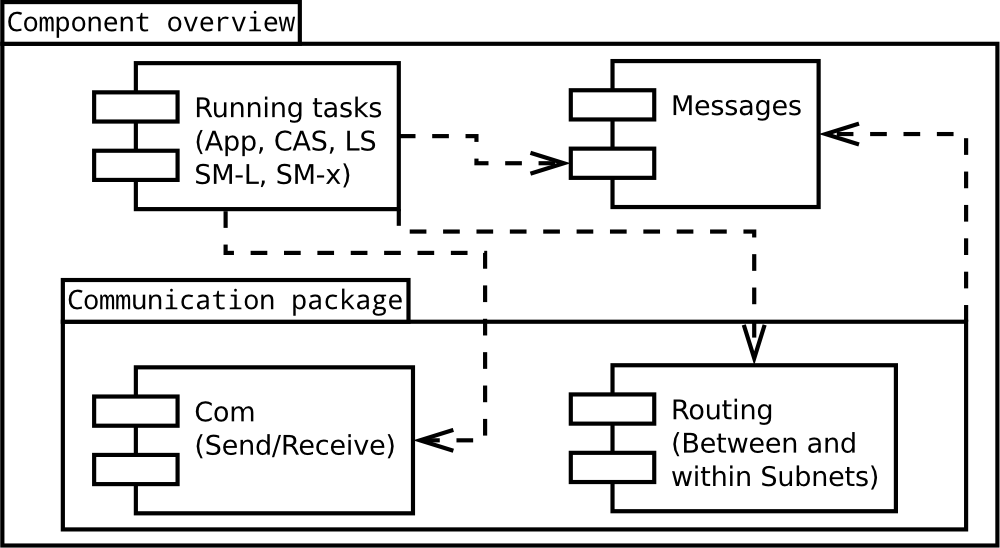
\includegraphics[width=\textwidth]{figures/iteration2_uml_component_overview}
    \caption{Component overview of a basic SPA implementation}
    \label{fig:iteration2_uml_component_overview}
\end{figure}

The design of the Communication package make use of the "Composite
pattern" where Routing objects and Com objects all inherit from the same
interface and where the Routing objects are of composite types. Figure
\ref{fig:iteration2_difference} shows the difference between a simple
application and the SM-L. The use of the composite pattern makes it possible
for a "Running task" in the application layer to easily swap out how it
connects to one or multiple networks.

\begin{figure}[h]
    \begin{subfigure}[b]{0.5\linewidth}
        \centering
            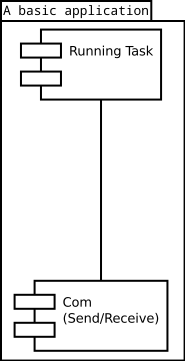
\includegraphics[width=0.9\textwidth]{figures/iteration2_uml_basic_application}
            \caption{An application}
            \label{fig:iteration2_uml_basic_application}
            \end{subfigure}%
        \begin{subfigure}[b]{.5\linewidth}
            \centering
            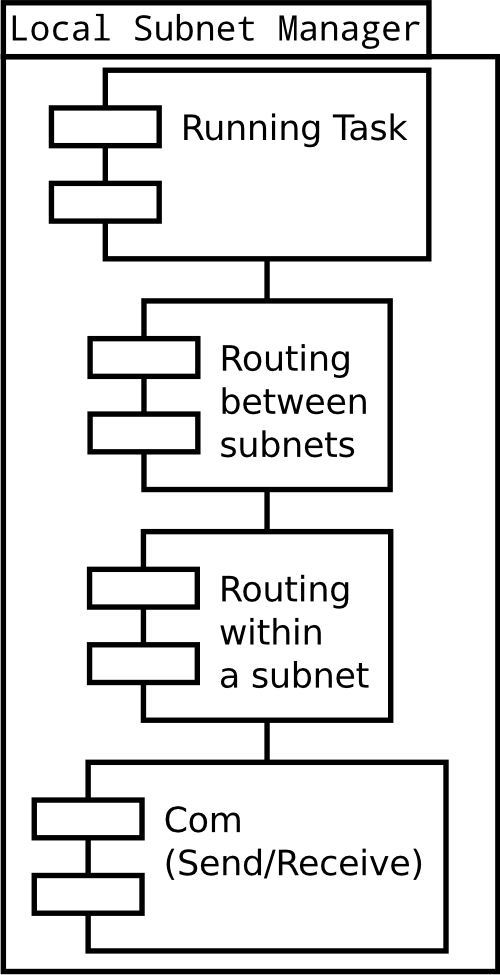
\includegraphics[width=0.9\textwidth]{figures/iteration2_uml_sm_l}
            \caption{A Subnet Manager}
            \label{fig:iteration2_uml_sm_l}
        \end{subfigure}
    \caption{The difference between a simple application and the SM-L.}
\label{fig:iteration2_difference}
\end{figure}

\subsubsection{A basic application}
TODO: The second iteration design has been presented, now improved UPPAAL
models must be shown.

\subsubsection{Central Addressing Service (CAS)}
TODO
\subsubsection{Lookup Service (LS)}
TODO
\subsubsection{Local Subnet Manager (SM-L)}
TODO
\subsubsection{Second iteration conclusions}
TODO

\section{Validation and Verification}
TODO: Add comments about time verification and correctness. What are the
verification lines used in UPPAAL to verify the system?

% \section{An event-triggered alternative}
% TODO: All models and comments about an event-triggered alternative.
